\documentclass[12pt]{article}
\usepackage{geometry}
\usepackage{color}
\usepackage{longtable}
\usepackage{graphicx}
\usepackage{amsmath,enumerate}
\usepackage{enumitem}
\usepackage{multirow}
\usepackage{amssymb}
\usepackage{float}
\usepackage{listings}
\lstset{
    breaklines = true
    }

\setenumerate[1]{itemsep=0pt,partopsep=0pt,parsep=\parskip,topsep=5pt}
\setitemize[1]{itemsep=0pt,partopsep=0pt,parsep=\parskip,topsep=5pt}
\setdescription{itemsep=0pt,partopsep=0pt,parsep=\parskip,topsep=5pt}
\usepackage{indentfirst}
\usepackage{float}
\usepackage{setspace}
\usepackage{pdfpages}
\usepackage{hyperref}
\usepackage{booktabs}
\geometry{a4paper,centering,scale=0.75} %a4paper

\linespread{1.4} %double spaced
\usepackage{amssymb, graphics, setspace}
\newcommand{\zdkh}[1]{\left\{\begin{aligned}#1\end{aligned}\right.}

\newcommand{\mathsym}[1]{{}}
\newcommand{\unicode}[1]{{}}

\newcommand{\tabincell}[2]{\begin{tabular}{@{}#1@{}}#2\end{tabular}}

\begin{document}
\thispagestyle{empty}
\vspace*{-2em}
\begin{figure}[H]
\centering

\includegraphics[width=0.8\textwidth]{LOGO}
\end{figure}
\vspace*{-2em}
\noindent \hrulefill
\vspace{12em}


\begin{center}

\begin{huge}
\sc{VE373 Design of Microprocessor Based Systems}
\end{huge}\\
\vspace*{1cm}
\begin{huge}
	\sc{Final Project Report}
\end{huge}\\
\vspace*{1cm}
\begin{huge}
	\sc{EMG Based PIC32 Musical Instrument}
\end{huge}\\

\vspace*{2cm}
\end{center}


\vfill
\noindent\hrulefill
\begin{table}[h!]
\flushleft
\begin{tabular}{lll}
Name: Zekun Du \hspace*{2em}&
Name: Yipai Du \hspace*{2em}&
Name: Tao Liang\hspace*{2em}\\
Date: August 10, 2017\\
\end{tabular}
\end{table}
\vspace{-4em}

\newpage
\tableofcontents

\newpage
\section{Objectives}

Nowadays, wearable devices are more and more popular. This brings a lot of joy and entertainment to people’s lives. The recent advancements in sensors enable us to acquire biomedical signals from human bodies and do analysis based on them, thus help to monitor the physical status of one person and trace one’s physical behavior. Motivated by this new trend, we are going to take advantage of the EMG signal processing technologies and implement a joyful musical instrument based on PIC32 MCU. 

Our project is called EMG based PIC32 musical instrument. It acquires muscle status with three EMG sensors. The analog signal is sent to the MCU and to the processing, including AD conversion, filtering and processing, to judge whether the muscle is at tension or not. With different combinations of the muscles’ status, we can identify which music note the user wants to play. The MCU then send the corresponding activate signal to the loudspeaker. Meanwhile, there are LED lights available to be turned on and off to add more fun to the music.


\section{Functional Blocks}
\begin{figure}[H]
\centering
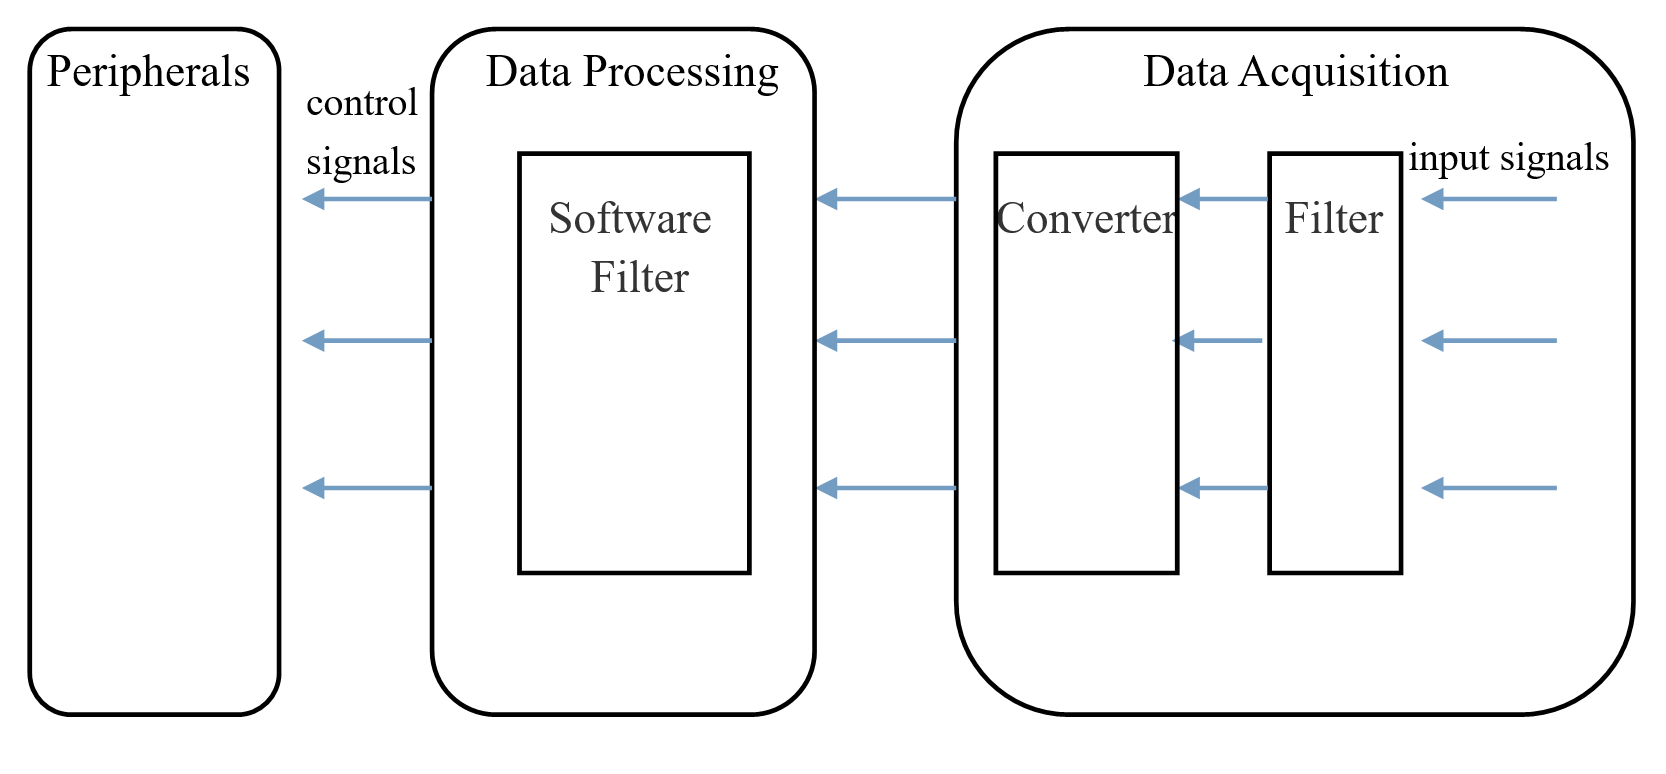
\includegraphics[width=0.6\textwidth]{block-diagram.png}
\caption{Functional Block Diagram.}
\end{figure}

Our project consists of three main parts: data acquision, data processing and output peripherals. In the data acquisition part, we use Arduino AD8232 as microcontroller which is responsible for filtering the signals sent by EMG sensors and then sending the processed analog data to PIC32 MCU. MUC will translate the analog signals to digital signals. We apply an external 9-volt battery to Arduino board as power supply.

Data processing part uses PIC32 MCU as microcontroller which can receive data from the data access part by DMA in real time. Since the hardware filter in data access part is not good enough, we will filter the input signals again by algorithm.

In the output peripherals part, PIC32 is connected with seven speakers which will generate seven different notes, and seven LEDs which represent the seven notes.


\section{Hardware Components}
\subsection{Data Acquisition Part}

\begin{figure}[H]
\centering
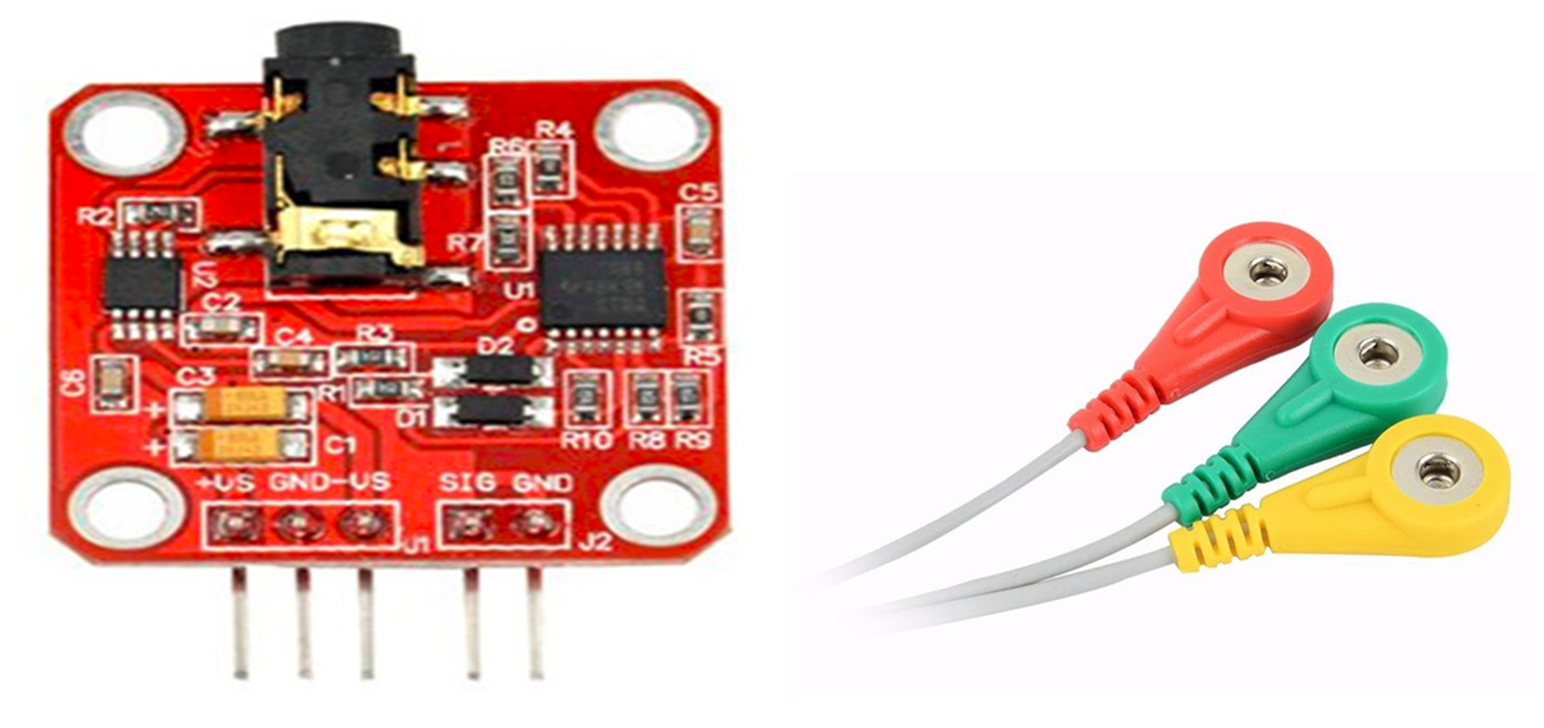
\includegraphics[width=0.8\textwidth]{sensor.png}
\caption{Arduino AD8232 and EMG sensors.}
\end{figure}

The combination of Arduino AD8232 and EMG sensors can detect and record the electrical signals produced by skeletal muscles. And the Arduino board can preliminarily filter the input signals. Moreover, to generate seven different notes, we need 3 sensors by arrangement.

\subsection{Data Processing Part}

\begin{figure}[H]
\centering
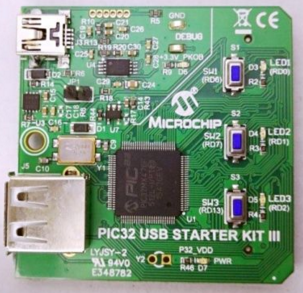
\includegraphics[width=0.4\textwidth]{pic32.png}
\caption{PIC32 Board.}
\end{figure}

We will use PIC 32 as the microcontroller to convert the input signals from analog singals to digital signals, denoise them and send the processed data to the output peripherals.

\begin{figure}[H]
\centering
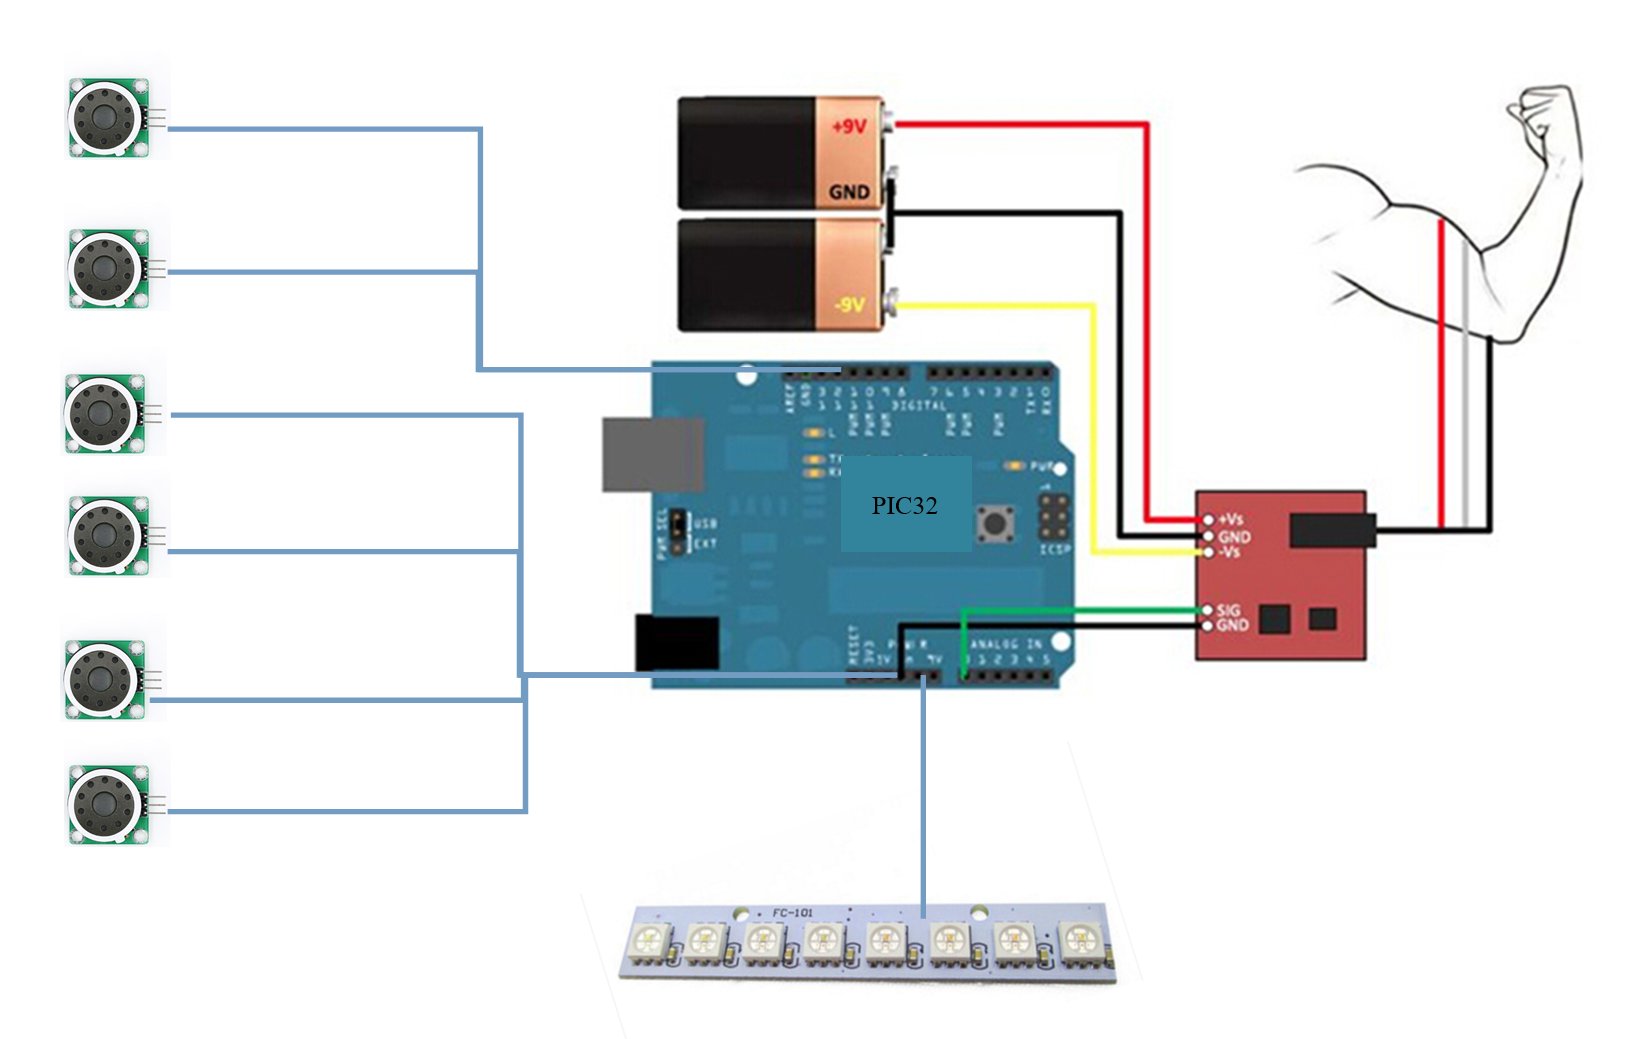
\includegraphics[width=0.6\textwidth]{hardware-diagram.png}
\caption{Components Diagram.}
\end{figure}

\newpage
\section{Embedded System Design}
\subsection{Data Acquisition Part}

In this part, I will use three functions to realize the data acqusition. ADCconfig() fucntion is used to config the ADC peripherals. In this project, we select the scan model to control three ADC pins in parrallel. Since we can not get the exact sampling rate by the formula provided by the data sheet, we will use tr4config() function to config the timer 4 to control the sampling rate. After we get the data, we will use DMAconfig() function to start the DMA channels.

\subsection{Digital Signal Processing part}
Thanks to the advantage of DMA module, the signal processing part is significantly simplified. Direct Memory Access allows us to transfer the array containing recently obtained voltage information to the correct position (called "receiver" in the program). Hence, the "receiver" in this case can always be assumed as the current value together with values of a short period before now. 

The purpose for digital signal processing part is basically to set three parameters. The first one is the proper threshold for identification of high and low voltage. The second parameter is the time interval of asynchronism that we want to synchronize. Notice that we are using the combination of status of three muscles to represent different notes. The rise of voltage from different muscles may not appear at the same time. Say the first muscle has a rising edge at time $t_1$, and later the second muscle has a rising edge at $t_2$. So the status at $t_1$ and $t_2$ should be different. The problem is when $t_2-t_1$ is too short, it should be considered as a noise. So the threshold is for measuring the interval $t_2-t_1$. If this threshold is set too short, not much noise can be filtered out. On the other hand, if it is too long, much delay will be introduced and causing a negative effect in the real time behavior. The third parameter is the size of the array of the accumulated status. If the array is set too large, more data to be processed will consume more CPU resource. If the array is too small, not much previous values is given for filtering noise, resulting inaccurate recognition of status. So basically the algorithm for digital signal processing part is simple enough to be implemented onto a PIC32 board. Most of the job is the onsite tuning of the parameters to make the system accurate as well as fast.

\subsection{PWM part}

This part is based on the handled data from the previous two parts. DSP part offers three bits (0 or 1) in the variable struct status refering to three sensors (A, B and C). We can calculate the combination of three signals to form 8 different result. We use PWM to generate a certain frequency of square waves representing the true sound wave. And send the wave to the speaker through the signal pin, so that we can play a note as we mentioned. The notes that signals refers to is shown below:

\begin{table}[H]
\centering
\begin{tabular}{cc}
(A, B, C) & Note \\\hline
(0, 0, 0) & Silence \\
(0, 0, 1) & C \\
(0, 1, 0) & D \\
(0, 1, 1) & E \\
(1, 0, 0) & F \\
(1, 0, 1) & G \\
(1, 1, 0) & A \\
(1, 1, 1) & B \\
\end{tabular}
\caption{Signal-Note Reference Table.}
\end{table} 

For specific functions, in speaker.h file: initIntGlobal() is used to enable multiple interrupt vectors; initPWM() is used to configerate basic bits of PWM mode, also in this PWM we use timer2 as reference; play() is the function we use to play a fixed note automatically according to the table above. 


\newpage
\section{Test Plan}
\subsection{Data Acquisition Part}

First, we needed to make sure the output signal of the EMG sensors should be inside the range of the reference voltage for ADC peripherals on pic32. We linked the output pin of the EMG sensors with the oscilloscope. Since the reference voltage set on the pic32 board is 3.3V, we finally adjusted the low signal of the sensor to about 1.1V and high signal to about 2.5V.

Second, we needed to know the exact sample rate of the ADC part to make it easier for the data processing part. At first, we just used the formula on the data sheet to calculate the sample rate, but we found that the calculated result was not exact. Then, to solve this problem, we used timer interrupt to control the sample rate. When timer interrupt is called, we converted the accepted data once.

Last, we wanted to test whether the DMA part works. We used the register watcher to monitor the destination registers of the DMA. Then we could know whether the data sampled by ADC were sent to the memory.

\subsection{Digital Signal Processing part}
The test for digital signal processing part is based on physical tuning of the parameters. The sampling time of the ADC module needs to be validated, so that we know the exact time that each voltage value corresponds to. Then based on the performance of the overall system, we try different sets of the three parameters. To our grief, the gain of the signal from the EMG sensors can also be adjusted, so we can adjust the three gains so the three signals can reach the same voltage level which will greatly simplify our task. 

The tuning of the parameters is seemingly easy, but consumes lots of time because we want to get an optimized performance, balancing accuracy and fastness. What beats us finally is the fastness and we decided to use a longer delay at around $0.5s$ to try to minimize the noise. This is because when playing a music, it not hurts to be a little bit slower but a single wrong note will influence a lot.

\subsection{PWM Part}

The PWM wave frequency is generated together by SYSCLK, PBDIV, prescale and PR2. So after we calculate and set appropriate data, we give different notes different PR2. To make sure the frequency of the sound wave is what we want, we use oscillator to measure the frequency. PWM needs 3.3V power supply so we connect the +pin to 3.3V pin on the board and -pin to the ground pin. We send the PWM wave through D pin which means digital signal.

\newpage
\section{Component List}
\begin{table}[H]
\centering
\begin{tabular}{ccc}
Peripheral Name &	Quantity &	Function\\ \hline
EMG sensors with driver boards	& 3	& \tabincell{c}{Sense the EMG signals and transmits\\to the PIC32 board.}\\
Speakers	& 1 &	\tabincell{c}{Give out sounds with the music notes’ \\frequencies to play a piece of song.} \\
\end{tabular}
\caption{Signal-Note Reference Table.}
\end{table} 


\section{Schedule}
\begin{figure}[H]
\centering
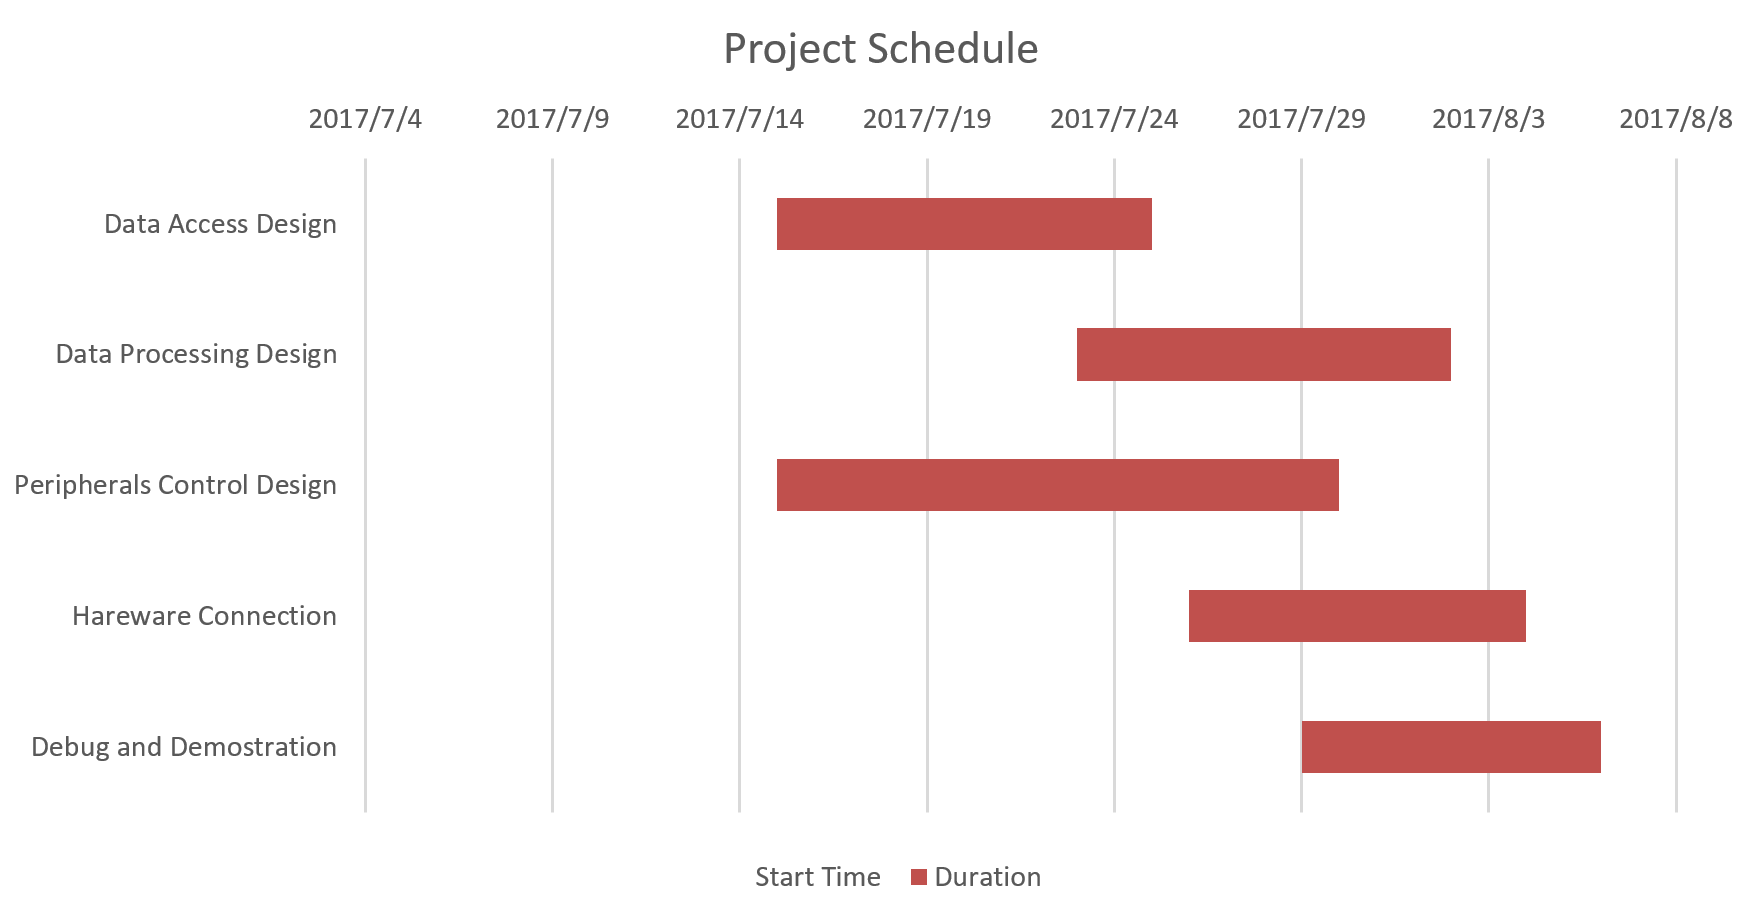
\includegraphics[width=0.7\textwidth]{Schedule.png}
\caption{Schedule.}
\end{figure}

Actually we follow this schedule and finish the program.

\section{Budget}
\begin{table}[H]
\centering
\begin{tabular}{|c|c|c|c|} 
\hline
Item	& Quantity &	Price(RMB) &	Hyperlink \\ \hline
EMG Sensors	 & 3   & 	 102.39	& \tabincell{c}{https://item.taobao.com/\\item.htm?scm=1007.10009.70205.1\\00200300000001\&id=53654844191\\5\&pvid=c144fb31-3bf3-44\\e7-8bf9-99647418a048} \\ \hline
Speaker	 & 1	& 10	& \tabincell{c}{https://item.taobao.com/i\\tem.htm?id=55094499545\\6\&ns=1\&abbucket=1\\9\#detail} \\ \hline
Total price	 &	& 317.17 & \\ \hline
\end{tabular}
\caption{Budget.}
\end{table} 

\newpage
\section{Appendix}

\textbf{dsp.h}

\lstset{language=C}
\begin{lstlisting}
#ifndef DSP_H
#define DSP_H
struct status
{
    unsigned char statusA;
    unsigned char statusB;
    unsigned char statusC;
};

struct Receiver
{
    unsigned char arrA[2];
    unsigned char arrB[2];
    unsigned char arrC[2];
} receiver;

void pushStatus();
struct status getNote();
#endif 
\end{lstlisting}

\textbf{speaker.h}

\lstset{language=C}
\begin{lstlisting}
#ifndef PWM_H
#define PWM_H
#include "dsp.h"
void T3Con(void);
void initIntGlobal(void);
void initPWM(void);
void play(struct status signal);
#endif
\end{lstlisting}


\textbf{acquisition.h}

\lstset{language=C}
\begin{lstlisting}
#ifndef ACQUISITION_H
#define ACQUISITION_H
#include <p32xxxx.h>

void ADCcSonfig(void);
void ADC_interrupt(void);
void DMAconfig();
void DMA0_ISR ();
void DMA1_ISR ();
void DMA2_ISR ();
#endif
\end{lstlisting}

\textbf{acquisition.c}
\lstset{language=C}
\begin{lstlisting}
#include "dsp.h"
#include <plib.h>
#include <sys/kmem.h>

static unsigned char valueA,valueB,valueC,nonidea;
static unsigned char arrA1[2];

static unsigned char arrA2[2];
static unsigned char arrB1[2];

static unsigned char arrB2[2];
static unsigned char arrC1[2];

static unsigned char arrC2[2];

static int count=0;

void DMAconfig();

void ADCcSonfig(void){
	asm ("ei"); 				// Enable all interrupts
/*	IPC6SET = 0x08000000; 		// Interrupt priority level 2, Subpriority level 0
	IFS1CLR = 0x00000002; 		// Clear timer interrupt flag
	IEC1SET = 0x00000002; 		// Enable ADC interrupt
*/
	TRISB = 0xffff;		//a. pin input
	AD1PCFG = 0xffc7;      //PORTB = Digital; RB3,4,5 = analog

//	AD1CHSbits.CH0SA = 0b0011;	//b.  AN3 as pos input
 // AD1CHSbits.CH0SB = 0b0011;	//b.  AN3 as pos input
	//AD1CON1bits = 0x000;		//c. set output format 000 (unsigned, frac, 16-bit)	
    AD1CON1bits.FORM=0b100;	
	AD1CON1SET = 0xE0;		//d. SSRC
	AD1CON2bits.VCFG = 0b011;	//e. VCFG 
	//AD1CON2SET = 0x400;		//f. CSCNA field of AD1CON2, MUX A
	//g. SMPI 0010
	AD1CON2bits.SMPI = 0b0010;
    //scan mode enable
    AD1CON2bits.CSCNA=0b1;
    //select scan pins,an3,an4,an5
    AD1CSSLSET=0x38;
	//h. BUFM
	AD1CON2CLR = 0x01;
	//i. ALTS (which MUX)
//	AD1CON2CLR = 0x0;
 	//j. ADRC		Tad > 65ns
	AD1CON3CLR = 0x8000;
	//k. SAMC auto-sample time bits 5
	AD1CON3bits.SAMC = 0b0101;
	//l. ADCS Tad = 50 Tpb -> ADCS = 24
	AD1CON3SET = 0x19;

	//m. turn on
	AD1CON1SET = 0x8000;
	AD1CON1bits.ASAM = 1;
}

/*#pragma interrupt ADC_interrupt ipl2 vector 27
void ADC_interrupt(void){
	//AD1CON1SET = 0x1;

	// deliver data to LCD
    if(count>=9)
    {
     	AD1CON1bits.SAMP = 0;
    }

    if(ADC1BUF0>=0b1100000000)
    {
     valueA=0b11111010;
     nonidea=ADC1BUF0;
     }
	else
    {
valueA=(330*ADC1BUF0)/1024;
nonidea=ADC1BUF0;
}
    
    if(ADC1BUF1>=0b1100000000)
    {
     valueB=0b11111010;
nonidea=ADC1BUF1;
     }
	else
    {valueB=(330*ADC1BUF1)/1024;
nonidea=ADC1BUF1;} 
 
    if(ADC1BUF2>=0b1100000000)
    {
     valueC=0b11111010;
nonidea=ADC1BUF2;
     }
	else
    {valueC=(330*ADC1BUF2)/1024;
nonidea=ADC1BUF2;}   

    arrA1[count]=valueA;
    arrB1[count]=valueB;
    arrC1[count]=valueC;
    count++;

	if(count>=10)
     {
		int i1;
		for(i1=0;i1<=9;i1++)
		{
		arrA2[i1]=arrA1[i1];
		}
		for(i1=0;i1<=9;i1++)
		{
		arrB2[i1]=arrB1[i1];
		}
		for(i1=0;i1<=9;i1++)
		{
		arrC2[i1]=arrC1[i1];
		}
		count=0;
		DMAconfig();

		
		DCH0ECONSET=0x00000080;//SET CFORCE to be 1 to start dma transfer
		DCH1ECONSET=0x00000080;//SET CFORCE to be 1 to start dma transfer
		DCH2ECONSET=0x00000080;//SET CFORCE to be 1 to start dma transfer
		AD1CON1bits.SAMP = 1;
    }
	
	IFS1CLR = 0x2; 		// Clear ADC interrupt flag
}
*/
void DMAconfig()
{
IFS1CLR=0x00010000; // clear existing DMA channel 0 interrupt flag
IFS1CLR=0x00020000; // clear existing DMA channel 1 interrupt flag
IFS1CLR=0x00040000; // clear existing DMA channel 2 interrupt flag
DMACONSET=0x00008000; // enable the DMA controller
DCH0CON=0x3; // channel 0 disabled, priority 3, no chaining
DCH1CON=0x3; // channel 1 disabled, priority 3, no chaining
DCH2CON=0x3; // channel 2 disabled, priority 3, no chaining
DCH0ECON=0; // no start or stop IRQ, no pattern match
DCH1ECON=0; // no start or stop IRQ, no pattern match
DCH2ECON=0; // no start or stop IRQ, no pattern match
/********* program the transfer *********/
DCH0SSA=KVA_TO_PA(&arrA2[0]); // transfer source physical address
DCH0DSA=KVA_TO_PA(&(receiver.arrA[0])); // transfer destination physical address
DCH0SSIZ=2; // source size 30 bytes
DCH0DSIZ=2; // destination size 30 bytes
DCH0CSIZ=2; // 30 bytes transferred per event
DCH1SSA=KVA_TO_PA(&arrB2[0]); // transfer source physical address
DCH1DSA=KVA_TO_PA(&(receiver.arrB[0])); // transfer destination physical address
DCH1SSIZ=2; // source size 30 bytes
DCH1DSIZ=2; // destination size 30 bytes
DCH1CSIZ=2; // 30 bytes transferred per event
DCH2SSA=KVA_TO_PA(&arrC2[0]); // transfer source physical address
DCH2DSA=KVA_TO_PA(&(receiver.arrC[0])); // transfer destination physical address
DCH2SSIZ=2; // source size 30 bytes
DCH2DSIZ=2; // destination size 30 bytes
DCH2CSIZ=2; // 30 bytes transferred per event
DCH0INTCLR=0x00ff00ff; // clear existing events, disable all interrupts
DCH0INTbits.CHBCIE=1;//enable the destination done interrupt
DCH1INTCLR=0x00ff00ff; // clear existing events, disable all interrupts
DCH1INTbits.CHBCIE=1;//enable the destination done interrupt
DCH2INTCLR=0x00ff00ff; // clear existing events, disable all interrupts
DCH2INTbits.CHBCIE=1;//enable the destination done interrupt
IPC9CLR=0x0000001f; // clear the DMA channel 0 priority and sub-priority
IPC9SET=0x00000006; // set IPL 1, sub-priority 2
IPC9CLR=0x00001F00; // clear the DMA channel 1 priority and sub-priority
IPC9SET=0x00000600; // set IPL 1, sub-priority 2
IPC9CLR=0x001F0000; // clear the DMA channel 2 priority and sub-priority
IPC9SET=0x00060000; // set IPL 1, sub-priority 2
IEC1SET=0x00010000; // enable DMA channel 0 interrupt
IEC1SET=0x00020000; // enable DMA channel 1 interrupt
IEC1SET=0x00040000; // enable DMA channel 2 interrupt
DCH0CONSET=0x80; // turn channel on
DCH1CONSET=0x80; // turn channel on
DCH2CONSET=0x80; // turn channel on
}

#pragma interrupt DMA0_ISR ipl1 vector 36
void DMA0_ISR ()
{
IFS1CLR=0x00010000; // clear existing DMA channel 0 interrupt flag
//DCH0ECONbits.CABORT=0b1;
//pushStatus();
}

#pragma interrupt DMA1_ISR ipl1 vector 37
void DMA1_ISR ()
{
IFS1CLR=0x00020000; // clear existing DMA channel 1 interrupt flag
//DCH1ECONbits.CABORT=0b1;
//pushStatus();
}

#pragma interrupt DMA2_ISR ipl1 vector 38
void DMA2_ISR ()
{
IFS1CLR=0x00040000; // clear existing DMA channel 2 interrupt flag
//DCH2ECONbits.CABORT=0b1;
pushStatus();
}

#pragma interrupt T4_ISR ipl3 vector 16
void T4_ISR (void) {
 if(count>=1)
    {
     	AD1CON1bits.SAMP = 0;
    }

    if(ADC1BUF0>=0b1100000000)
    {
     valueA=0b11111010;
     nonidea=ADC1BUF0;
     }
	else
    {
valueA=(330*ADC1BUF0)/1024;
nonidea=ADC1BUF0;
}
    
    if(ADC1BUF1>=0b1100000000)
    {
     valueB=0b11111010;
nonidea=ADC1BUF1;
     }
	else
    {valueB=(330*ADC1BUF1)/1024;
nonidea=ADC1BUF1;} 
 
    if(ADC1BUF2>=0b1100000000)
    {
     valueC=0b11111010;
nonidea=ADC1BUF2;
     }
	else
    {valueC=(330*ADC1BUF2)/1024;
nonidea=ADC1BUF2;}   

    arrA1[count]=valueA;
    arrB1[count]=valueB;
    arrC1[count]=valueC;
    count++;

	if(count>=2)
     {
		int i1;
		for(i1=0;i1<=1;i1++)
		{
		arrA2[i1]=arrA1[i1];
		}
		for(i1=0;i1<=1;i1++)
		{
		arrB2[i1]=arrB1[i1];
		}
		for(i1=0;i1<=1;i1++)
		{
		arrC2[i1]=arrC1[i1];
		}
		count=0;
		DMAconfig();

		
		DCH0ECONSET=0x00000080;//SET CFORCE to be 1 to start dma transfer
		DCH1ECONSET=0x00000080;//SET CFORCE to be 1 to start dma transfer
		DCH2ECONSET=0x00000080;//SET CFORCE to be 1 to start dma transfer
		AD1CON1bits.SAMP = 1;
    }
IFS0CLR = 0x0010000; // Clear timer 4 interrupt flag
}

void tr4config()
{
	IPC4SET = 0x0000000C; //Set priority level = 3
	IPC4SET = 0x00000001; //Set subpriority level = 1
	IFS0CLR = 0x00010000; //Clear Timer interrupt flag
	IEC0SET = 0x00010000; //Enable Timer interrupts

	T4CON = 0x0; // Stop any 16/32-bit Timer2 operation
	T4CONbits.TCKPS =  0B010; // Enable 16-bit mode, prescaler 1:1,
                    // internal clock
	TMR4 = 0x0; // Clear contents of TMR2
	PR4=1200;
	T4CONSET = 0x8000;
}
\end{lstlisting}

\textbf{dsp.c}

\lstset{language=C}
\begin{lstlisting}
#include "dsp.h"
static unsigned char threshold = 100;
static unsigned char numOfHit(struct accumStatus * arr, struct status * element, unsigned char index);
static unsigned char statusEq(struct status * a, struct status * b);
struct accumStatus
{
    struct status statusArr[20];
    unsigned char size;
    unsigned char frontIndex;
};

static struct status nullStatus;
struct accumStatus globalStatus;

struct status getNote()
{
    if (globalStatus.size<19)
    {
        return nullStatus;
    }
    else
    {
        if (numOfHit(&(globalStatus.statusArr), &(globalStatus.statusArr[globalStatus.frontIndex]), globalStatus.frontIndex)>18)
        {
            nullStatus = globalStatus.statusArr[globalStatus.frontIndex];
            return globalStatus.statusArr[globalStatus.frontIndex];
        }
        else
        {
            return nullStatus;
        }
    }
}

void pushStatus()
{
    struct status * modifiy = &(globalStatus.statusArr[globalStatus.frontIndex]);
    ++ globalStatus.size;
    ++globalStatus.frontIndex;
    if(globalStatus.frontIndex > 19)
    {
        globalStatus.frontIndex = 0;
    }

    unsigned char hit = 0;
    unsigned char i;
    for(i = 0; i < 2; ++i)
    {
        if(receiver.arrA[i] > threshold)
        {
            ++hit;
        }
    }
    if (hit ==2)
    {
        modifiy->statusA = 1;
    }
    else
    {
        modifiy->statusA = 0;
    }

    hit = 0;
    for(i = 0; i < 2; ++i)
    {
        if(receiver.arrB[i] > threshold)
        {
            ++hit;
        }
    }
    if (hit == 2)
    {
        modifiy->statusB = 1;
    }
    else
    {
        modifiy->statusB = 0;
    }

    hit = 0;
    for(i = 0; i < 2; ++i)
    {
        if(receiver.arrC[i] > threshold)
        {
            ++hit;
        }
    }
    if (hit == 2)
    {
        modifiy->statusC = 1;
    }
    else
    {
        modifiy->statusC = 0;
    }
}

static unsigned char statusEq(struct status * a, struct status * b)
{
    unsigned char res = 0;
    if(a->statusA == b->statusA)
    {
        if(a->statusB == b->statusB)
        {
            if(a->statusC == b->statusC)
            {
                res = 1;
            }
        }
    }
    return res;
}

static unsigned char numOfHit(struct accumStatus * arr, struct status * element, unsigned char index)
{
    unsigned char num = 0;
    unsigned char i=index-1;
    if (i<0)
    {
        i = 19;
    }
    while(statusEq(&(arr->statusArr[i]), element))
    {
        ++num;
        --i;
        if (i<0)
        {
            i=19;
        }
        if (i== index)
        {
            break;
        }
    }
/*
    for(i= 0; i < 20; ++i)
    {
        if(statusEq(&(arr->statusArr[i]), element))
        {
            ++num;
        }
    }*/
    return num;
}
\end{lstlisting}

\textbf{speaker.c}

\lstset{language=C}
\begin{lstlisting}
#include <p32xxxx.h>
#include <plib.h>
#include "dsp.h"
#include "speaker.h"

/*
In this file, components are used to fit FRCDIV (4MHz)
*/

/* Global variables */
static unsigned int flags = 0;
//static unsigned int flag_T2 = 0;

static unsigned int c3 = 3816;
static unsigned int d3 = 3400;
static unsigned int e3 = 3029;
static unsigned int f3 = 2864;
static unsigned int g3 = 2550;
static unsigned int a3 = 2272;
static unsigned int b3 = 2023;
static unsigned int c4 = 1911;
static unsigned int tmp = 1911;



/* Timer2 ISR - handling OC-PWM module operations */
#pragma interrupt PWM_ISR ipl3 vector 8
static void PWM_ISR (void) {
	OC1RS = PR2 * 0.12; //update duty cycle register
	IFS0CLR = 0x0100; //clear Timer 2 interrupt flag
}

/* Configure interrupt globally */
void initIntGlobal(void) {
	INTCONbits.MVEC = 1; // Enable multiple vector interrupt
	asm("ei"); // Enable all interrupts
}



/* Initialize OC module and timer base - Timer 2 */
void initPWM(void){
	OC1CON = 0x0000; //stop OC1 module
	OC1RS = 0; //initialize duty cycle register
	OC1R = 0; //initialize OC1R register for the first time
	OC1CON = 0x0006; //OC1 16-bit, Timer 2, in PWM mode w/o FP
	
	/*set frequency*/
	PR2 = tmp;

	IFS0CLR = 0x00000100; //clear Timer 2 interrupt	
	IEC0SET = 0x00000100; //enable Timer 2 interrupt
	IPC2SET = 0x0000000F; //Timer 2 interrupt priority 3, subpriority 3
	T2CONbits.TCKPS = 0b000; 	// prescale = 1:64
	T2CONSET = 0x8000; //start Timer 2
	OC1CONCLR = 0x8000; //enable OC1 module for PWM generation
}


static void note(unsigned int n){
	PR2 = n;
	OC1CONSET = 0x8000;
}


static void TestPWMFrequency(void){
	note(d3);
}

void play(struct status signal){
	if (signal.statusA == 0 && signal.statusB == 0 && signal.statusC == 0){
		OC1CONCLR = 0x8000;
	}
	else if(signal.statusA == 0 && signal.statusB == 0 && signal.statusC == 1){
		note(c3);
	}
	else if(signal.statusA == 0 && signal.statusB == 1 && signal.statusC == 0){
		note(d3);
	}
	else if(signal.statusA == 0 && signal.statusB == 1 && signal.statusC == 1){
		note(e3);
	}
	else if(signal.statusA == 1 && signal.statusB == 0 && signal.statusC == 0){
		note(f3);
	}
	else if(signal.statusA == 1 && signal.statusB == 0 && signal.statusC == 1){
		note(g3);
	}
	else if(signal.statusA == 1 && signal.statusB == 1 && signal.statusC == 0){
		note(a3);
	}
	else if(signal.statusA == 1 && signal.statusB == 1 && signal.statusC == 1){
		note(b3);
	}

}


\end{lstlisting}
\end{document}